% 2021_national_paper_a_science_q8_fig1: triangular elevation schematic
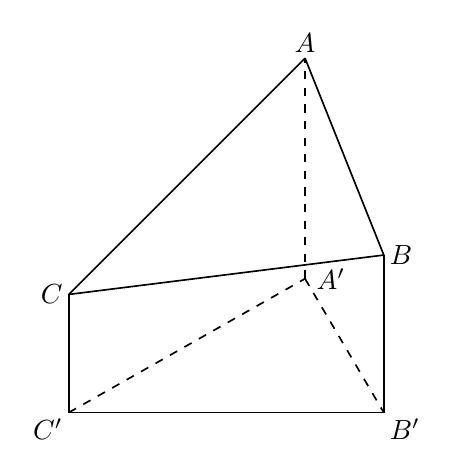
\begin{tikzpicture}[x=1cm,y=1cm,font=\normalsize,
  geometry edge/.style={solid,line width=.6pt},
  geometry label/.style={font=\normalsize,inner sep=2pt}]
\coordinate (A) at (3.5,5);
\coordinate (B) at (4.5,2.5);
\coordinate (C) at (0.5,2);
\coordinate (Ap) at (3.5,2.2);
\coordinate (Bp) at (4.5,0.5);
\coordinate (Cp) at (0.5,0.5);
\draw[geometry edge] (Cp)--(Bp);
\draw[geometry edge] (Cp)--(C);
\draw[geometry edge] (Bp)--(B);
\draw[geometry edge,dashed] (Ap)--(A);
\draw[geometry edge,dashed] (Cp)--(Ap);
\draw[geometry edge,dashed] (Ap)--(Bp);
\draw[geometry edge] (C)--(B);
\draw[geometry edge] (C)--(A);
\draw[geometry edge] (A)--(B);
\node[geometry label,above] at (A) {$A$};
\node[geometry label,right] at (B) {$B$};
\node[geometry label,left] at (C) {$C$};
\node[geometry label,right,xshift=2.00bp,yshift=0.00bp] at (Ap) {$A'$};
\node[geometry label,below right] at (Bp) {$B'$};
\node[geometry label,below left] at (Cp) {$C'$};
\end{tikzpicture}
